\chapter{\uppercase{PROSPECT Analysis Framework and Performance}}

Physics events in the PROSPECT detector, such as neutron captures on $^6$Li, produce scintillation light through ionization that is transported by way of the reflecting panels to individual PMTs. 
As described in Section~\ref{sec:DAQ}, these signals are processed by CAEN waveform digitizers and are only accepted if they pass the segment and ZLE thresholds.
Due to the nature of the liquid scintillator the shape of the digitized waveforms is defined by the 

\begin{figure}[h]
	\centering
	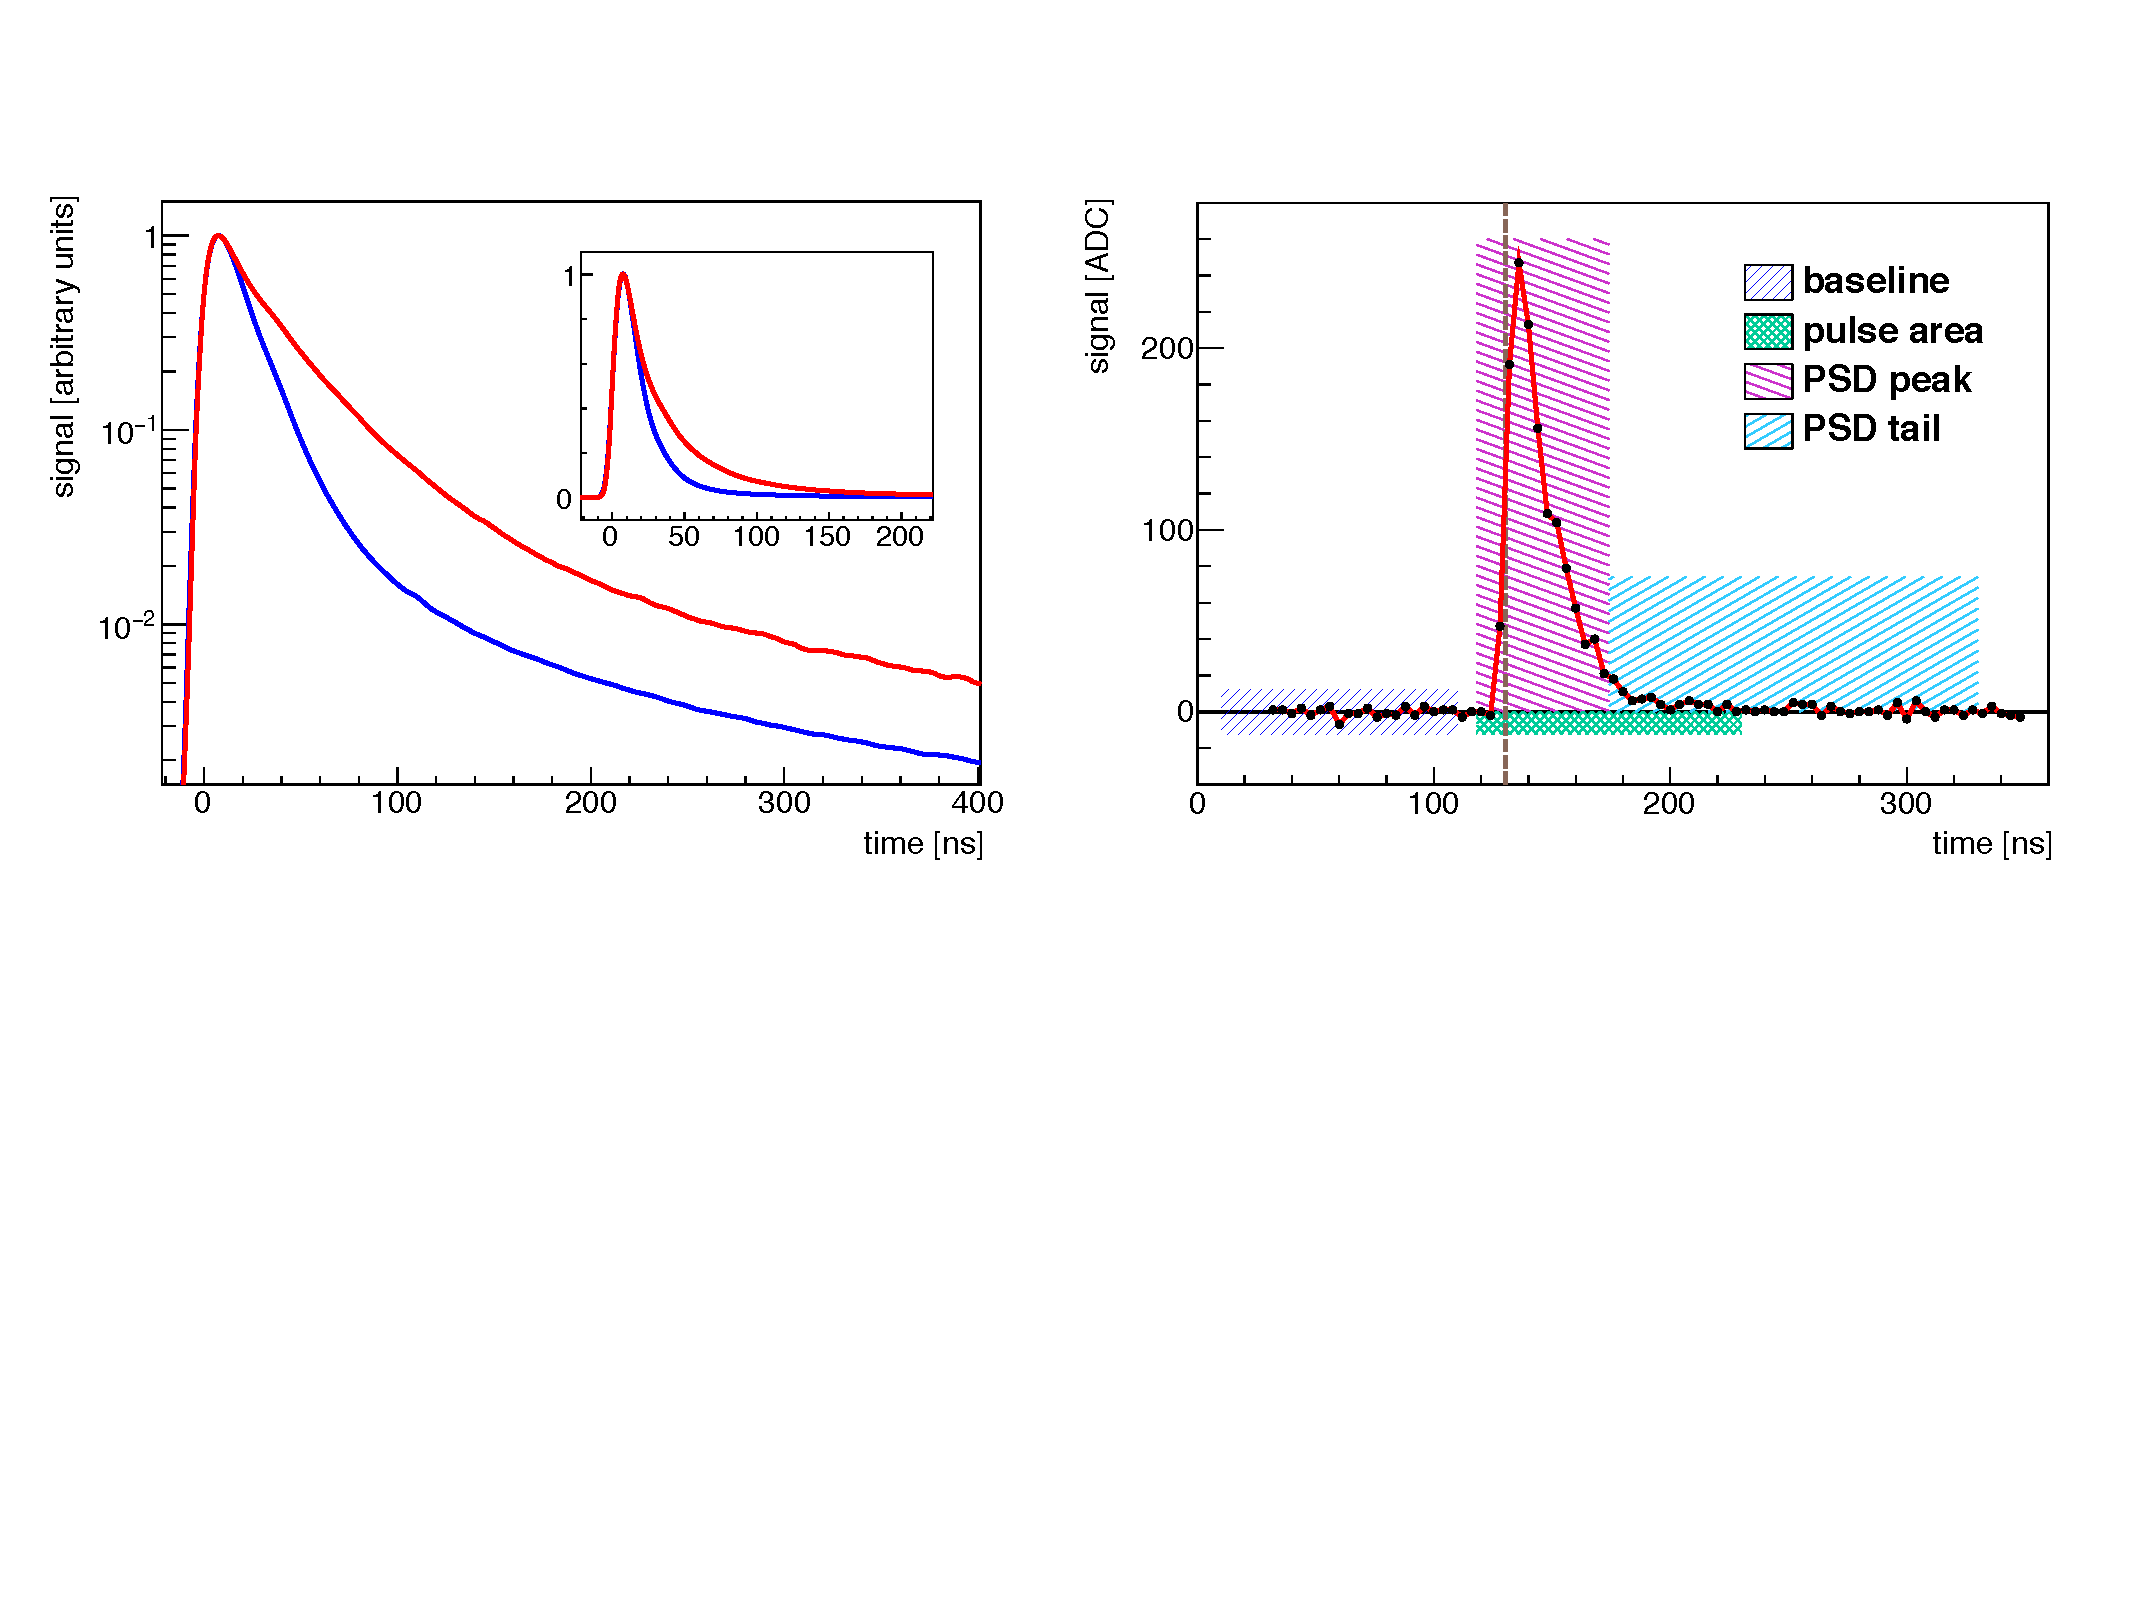
\includegraphics[width=0.99\linewidth]{tex/5-analysis-images/PSD_Define}
	\caption{(Left) Averaged waveforms from electrons (lower, blue) and proton recoils (upper, red). The inset panel shows the same waveforms on a linear y axis. (Right) Example analysis of a typical pulse. The half-height leading edge timing (dashed vertical) determines windows for baseline subtraction, pulse area, and PSD. }
	\label{fig:psddefine}
\end{figure}


\begin{figure}[h]
	\centering
	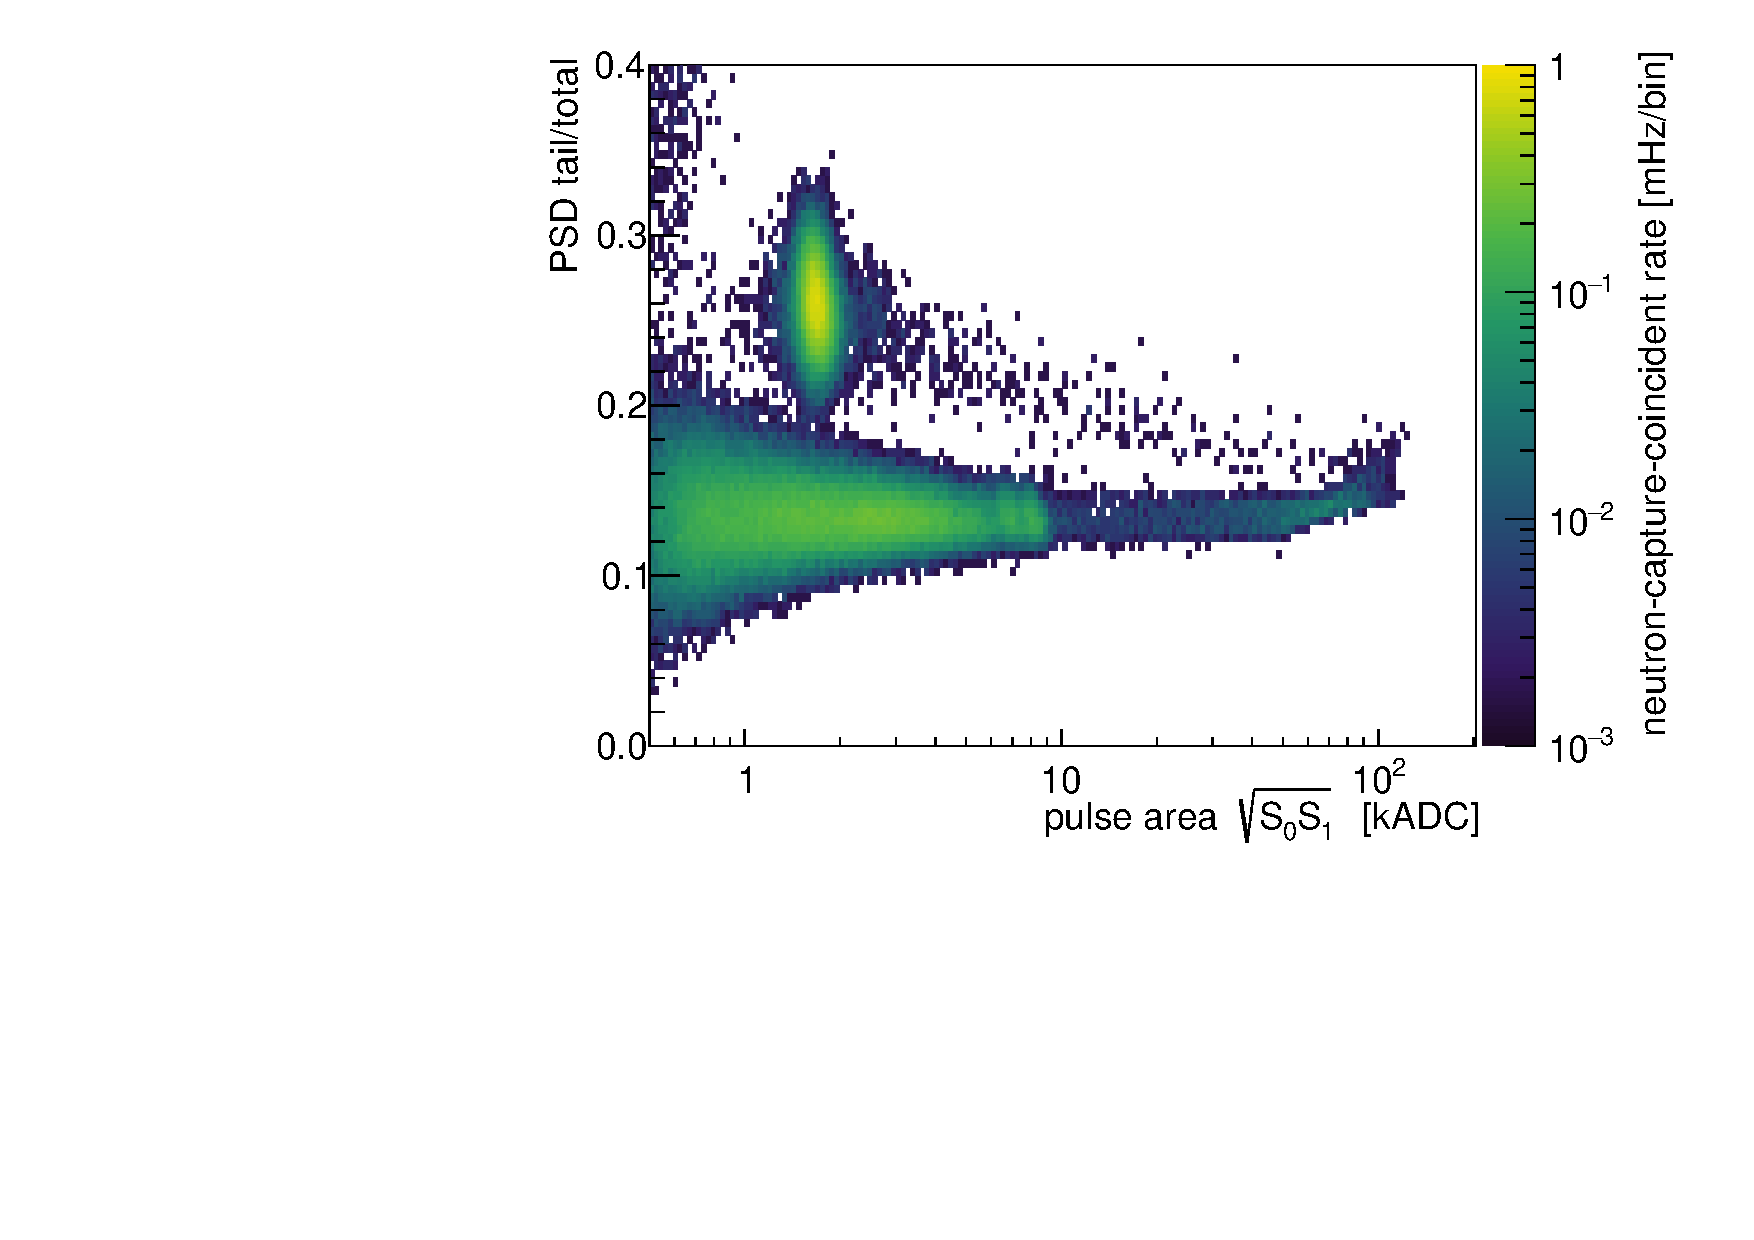
\includegraphics[width=0.7\linewidth]{tex/5-analysis-images/PSD_vs_S}
	\caption{}
	\label{fig:psdvss}
\end{figure}

